\documentclass[12pt, letterpaper]{report}
\usepackage[margin=1in]{geometry}
\usepackage[utf8]{inputenc}
\usepackage{graphicx}
\usepackage{amsmath}
\usepackage{float}
\usepackage{subfig}
\graphicspath{ {./img/} }
\setlength\parindent{0pt}
\renewcommand\thesection{\Roman{section}.}
\renewcommand{\thesubsection}{\alph{subsection}.}


\title{CS1675 - Assignment 4}
\author{Zachary M. Mattis}


\begin{document}
	
\maketitle

\section{Problem 1 - Data Analysis}

% A
\subsection{Binary Attributes}

There is only 1 binary attribute, \#4 CHAS. It is a Charles River dummy variable indicating if the housing tract bounds the river.

% B
\subsection{Correlations}

The attribute that demonstrated the highest positive correlation was \#6, RN, with a value of 0.6954. The attribute that demonstrated the highest negative correlation was \#13, LSAT, with a value of -0.7377.

\begin{table}[H]
	\centering
	\begin{tabular}{ |l|r| }
		\hline
		Attribute & Correlation \\
		\hline
		CRIM & -0.3883 \\
		\hline
		ZN & 0.3604 \\
		\hline
		INDUS & -0.4837 \\
		\hline
		CHAS & 0.1753 \\
		\hline
		NOX & -0.4273 \\
		\hline
		RM & 0.6954 \\
		\hline
		AGE & -0.3770 \\
		\hline
		DIS & 0.2499 \\
		\hline
		RAD & -0.3816 \\
		\hline
		TAX & -0.4685 \\
		\hline
		PTRATIO & -0.5078 \\
		\hline
		B & 0.3335 \\
		\hline
		LSTAT & -0.7377 \\
		\hline
	\end{tabular}
	\caption{Correlations}
\end{table}

% C
\subsection{Linear / Non-Linear}

The most correlated non-linear graph appears to be attribute 13, LSTAT. The data points are very closely packed, while the shape is not necessarily linear. The shape appears to be a quadratic function. It also has the highest negative correlation coefficient.

\begin{figure}[H]
	\centering
	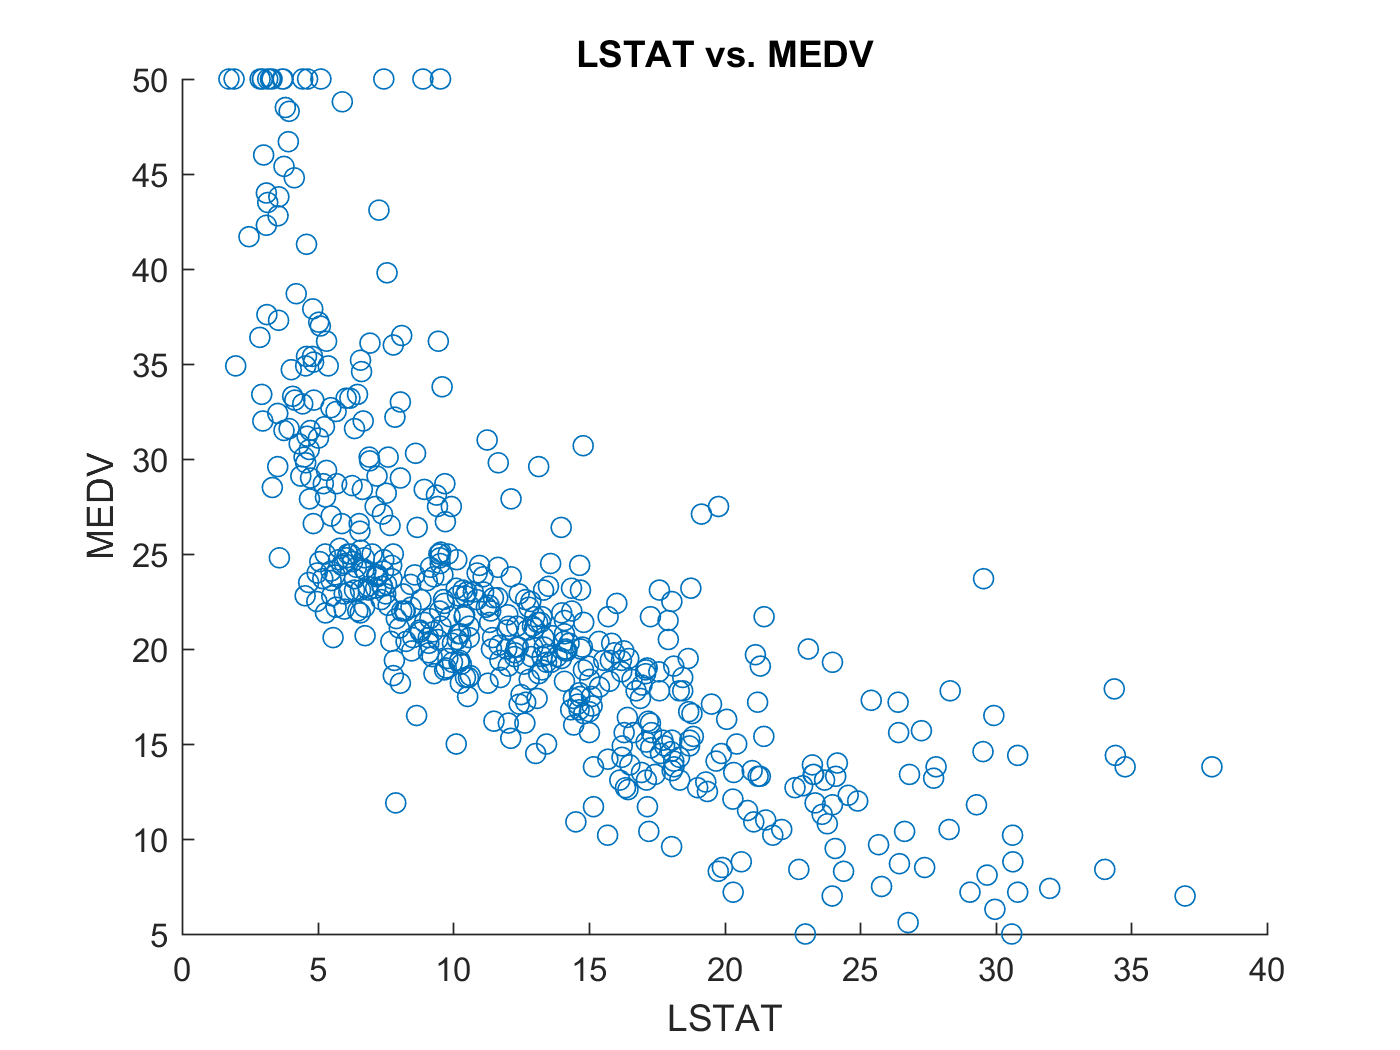
\includegraphics[width=0.7\columnwidth]{p1c13.png}
	\caption{Non-Linear}
\end{figure}

The most correlated linear graph appears to be attribute 6, RM.  In this case, there are a few outliers, but many points are located very close to a line of best fit. It also has the highest positive correlation coefficient.

\begin{figure}[H]
\centering
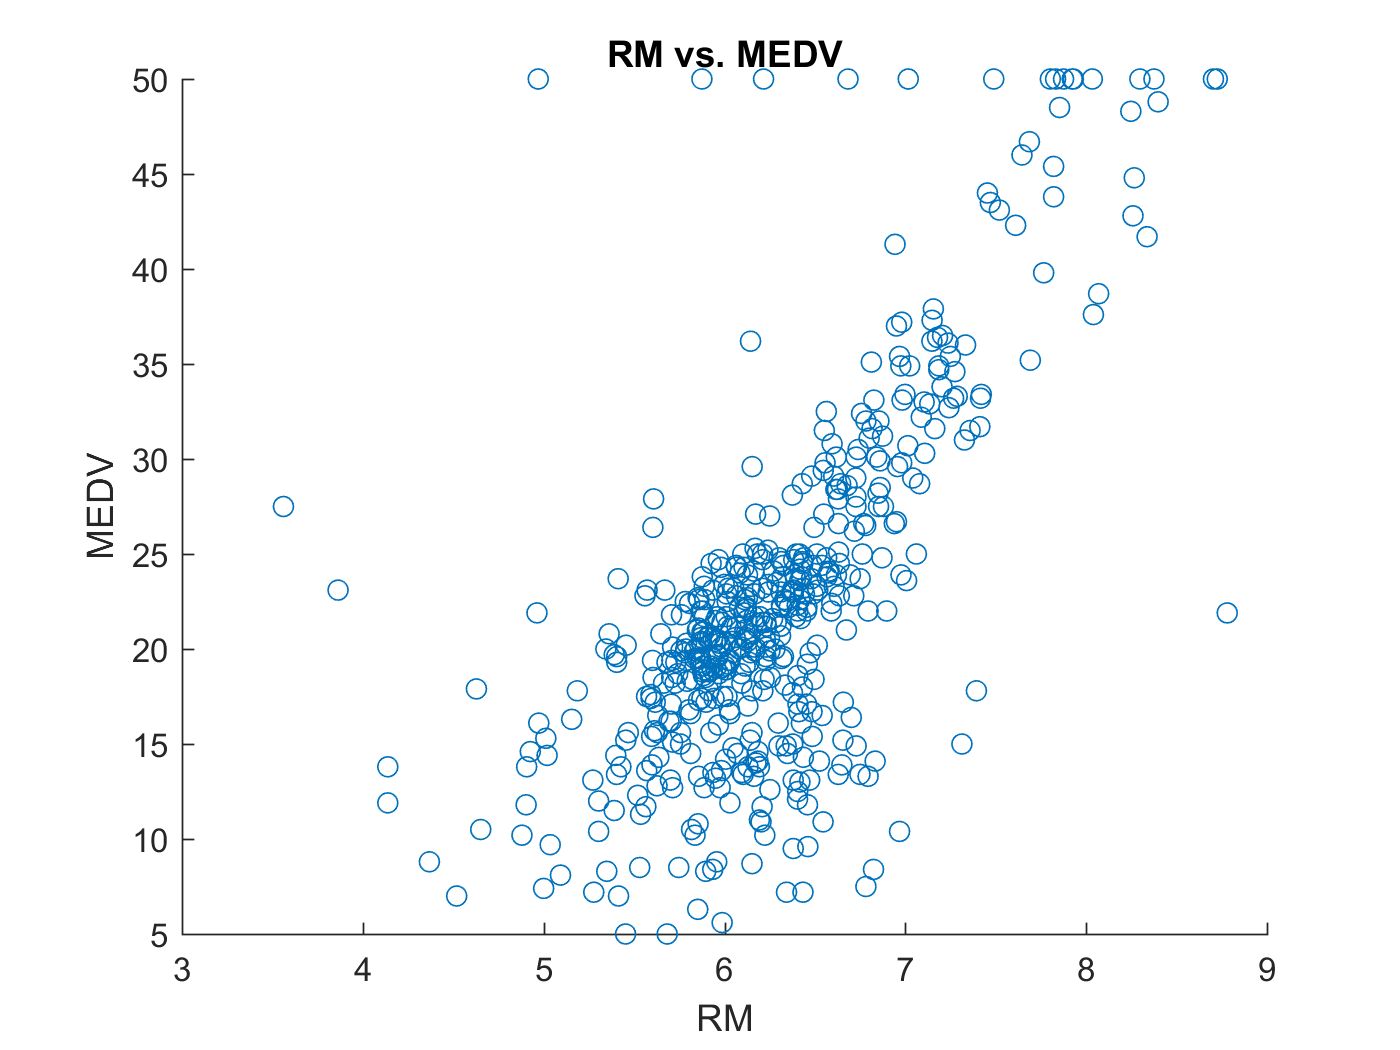
\includegraphics[width=0.7\columnwidth]{p1c6.png}
\caption{Linear}
\end{figure}

% D
\subsection{Mutual Correlation}

Attribute \#9, RAD, and attribute \#10, TAX, have the highest mutual correlation with a coefficient of 0.910228.

\section{Problem 2 - Linear Regression}

% A
\subsection{Solve}

\begin{verbatim}
function [ w ] = LR_solve( X, y )
    w = X\y;
end
\end{verbatim}

% B
\subsection{Predict}

\begin{verbatim}
function [ y ] = LR_predict( X, w )
    y = X*w;
end
\end{verbatim}

% C
\subsection{Training / Testing Data}

\[ MSE = \frac{1}{N} \sum (f_i -y_i)^2 \]

% D
\subsection{Weight / Mean Squared Error}

\begin{table}[H]
	\centering
	\begin{tabular}{ |l|r| }
		\hline
		Attribute & Weight \\
		\hline
		CRIM & -0.0979 \\
		\hline
		ZN & 0.0490 \\
		\hline
		INDUS & -0.0254 \\
		\hline
		CHAS & 3.4509 \\
		\hline
		NOX & -0.3555 \\
		\hline
		RM & 5.8165 \\
		\hline
		AGE & -0.0033 \\
		\hline
		DIS & -1.0205 \\
		\hline
		RAD & 0.2266 \\
		\hline
		TAX & -0.0122 \\
		\hline
		PTRATIO & -0.3880 \\
		\hline
		B & 0.0170 \\
		\hline
		LSTAT & -0.4850 \\
		\hline
	\end{tabular}
	\caption{LR Weights}
\end{table}

The mean squared error of the training data was 24.4759, while the MSE of the testing data was 24.2922. Because the MSE of the testing data was lower, this appears to be the better set, although they are both very close.

\section{Problem 3 - Online Gradient Descent}

% A
\subsection{Regression Coefficients}

\begin{verbatim}
online_gradient_descent.m
\end{verbatim}

% B
\subsection{Gradient Procedure}

The mean squared error of the training data was 34.2648, while the MSE of the testing data was 68.2374. In this particular case, the end result was worse than be solving the problem exactly.

\begin{table}[H]
	\centering
	\begin{tabular}{ |l|r| }
		\hline
		Attribute & Weight \\
		\hline
		CRIM & 0.2343 \\
		\hline
		ZN & 2.0068 \\
		\hline
		INDUS & 0.4363 \\
		\hline
		CHAS & -0.3487 \\
		\hline
		NOX & 8.5354 \\
		\hline
		RM & 1.358 \\
		\hline
		AGE & -5.4657 \\
		\hline
		DIS & 1.0777 \\
		\hline
		RAD & -4.7237 \\
		\hline
		TAX & 0.4721 \\
		\hline
		PTRATIO & 2.4667 \\
		\hline
		B & 2.6942 \\
		\hline
		LSTAT & -0.3014 \\
		\hline
	\end{tabular}
	\caption{OGD Weights}
\end{table}

% C
\subsection{No Normalization}

With un-normalized data, the weights approached infinity instantly.  Therefore, the weights and errors were not valid.

% D
\subsection{Data Observation}

\begin{figure}[H]
	\centering
	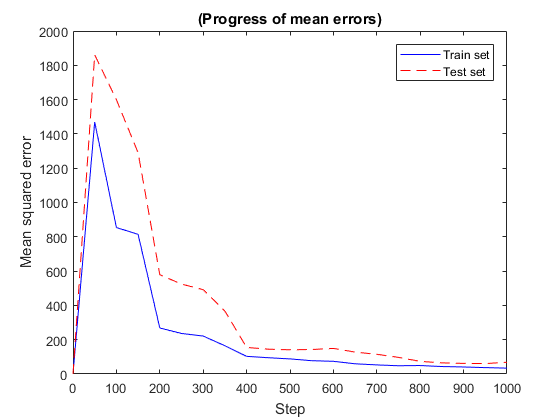
\includegraphics[width=0.7\columnwidth]{p3d.png}
	\caption{MSE}
\end{figure}

% E
\subsection{Trials}


\begin{table}[H]
	\centering
	\begin{tabular}{ |l|r|r|r|r|r|r|r|r| }
		\hline
		Steps & 1000 & 1000 & 1000 & 1000 & 1000 & 1000 & 10000 & 100000 \\
		\hline
		Learning Rate & 0.01 & 0.05 & $1/\sqrt{t}$ & $2/t^{2}$ & $2/t^{3}$ & 2/t & 2/t & 2/t \\
		\hline
		MSE Train & 0.2895 & 0.9875 & 3.66E+55 & 0.8247 & 0.5577 & 34.2648 & 5.3167 & 1.5551 \\
		\hline
		MSE Test & 0.1909 & 0.8354 & 4.27E+55 & 0.9502 & 0.5534 & 68.2374 & 8.4973 & 2.1502 \\
		\hline
		CRIM & -0.0639 & 0.4199 & -6.4E+27 & -0.1014 & -0.0684 & 0.2343 & 0.3515 & 0.1312 \\
		\hline
		ZN & 0.0383 & -0.1958 & 9.07E+26 & -0.1454 & -0.0823 & 2.0068 & 0.2848 & 0.0628 \\
		\hline
		INDUS & 0.0038 & 0.2318 & -5.8E+25 & 0.2605 & 0.0154 & 0.4363 & -0.6689 & -0.6397 \\
		\hline
		NOX & 0.2284 & 0.2222 & 1.34E+27 & 1.0100 & 0.5398 & 1.3580 & 1.1946 & 0.7857 \\
		\hline
		RM & -0.0005 & 0.2016 & -1.4E+27 & 0.1962 & -0.1313 & -5.4657 & -0.1862 & -0.7714\\
		\hline
		AGE & -0.1767 & -0.2337 & 6.56E+26 & -0.1858 & 0.0170 & 1.0777 & 0.5802 & 0.2096 \\
		\hline
		DIS & 0.1175 & 0.0543 & 1.58E+27 & -0.3084 & -0.1616 & -4.7237 & -2.6102 & -1.6003 \\
		\hline
		TAX & -00507 & -0.2419 & 4.12E+26 & -0.2002 & -0.1405 & 0.4721 & 0.9293 & 0.9607 \\
		\hline
		PTRATIO & -0.1213 & -0.0677 & -1.4E+26 & -0.2226 & -0.1121 & 2.4667 & 1.3450 & 0.5477 \\
		\hline
		B & 0.0385 & 0.0768 & -5.9E+25 & 0.0840 & 0.0449 & 2.6942 & 0.5061 & 0.2595 \\
		\hline
		LSTAT & -0.4389 & -0.3127 & 7.67E+26 & -0.2942 & -0.3686 & -0.3014 & -0.2189 & -0.2919 \\
		\hline
	\end{tabular}
	\caption{Trial Analysis}
\end{table}
	
Keeping the steps constant while changing the learning rate affects error the most.  The smaller the learning rate, the lower the error becomes.  It is likely that there is a threshold where a lower rate will have worse error (since the regression never approaches the optimum) if the number of steps are not enough.  If the learning rate is stalled, then the change becomes less noticeable as the function becomes “smaller and smaller” (such as $2/t^{2} => 2/t^{3}$).  Now, if the learning function remains the same while the steps increase, the errors go down with diminishing returns.

\end{document}